%! TEX rootmain.tex

\chapter{Discrete Systems}

Musical instruments can, at first glance, be described as assemblies of an exciter, a resonator and a sound emitter. In string instruments, for instance, the string is set into motion by plucking, striking or bowing; a bridge transmits energy to a resonant body and sound is radiated to the air. In wind instruments, airflow is perturbed (by a jet, reed or lip motion), shaped by the bore (the resonator) and emitted through the bell or tone holes. In all such examples, the organizing concept is oscillation, which is captured mathematically by harmonic motion.

\section{The Mass–Spring Model and the Harmonic Oscillator}

\begin{figure}[!htb]
    \centering
    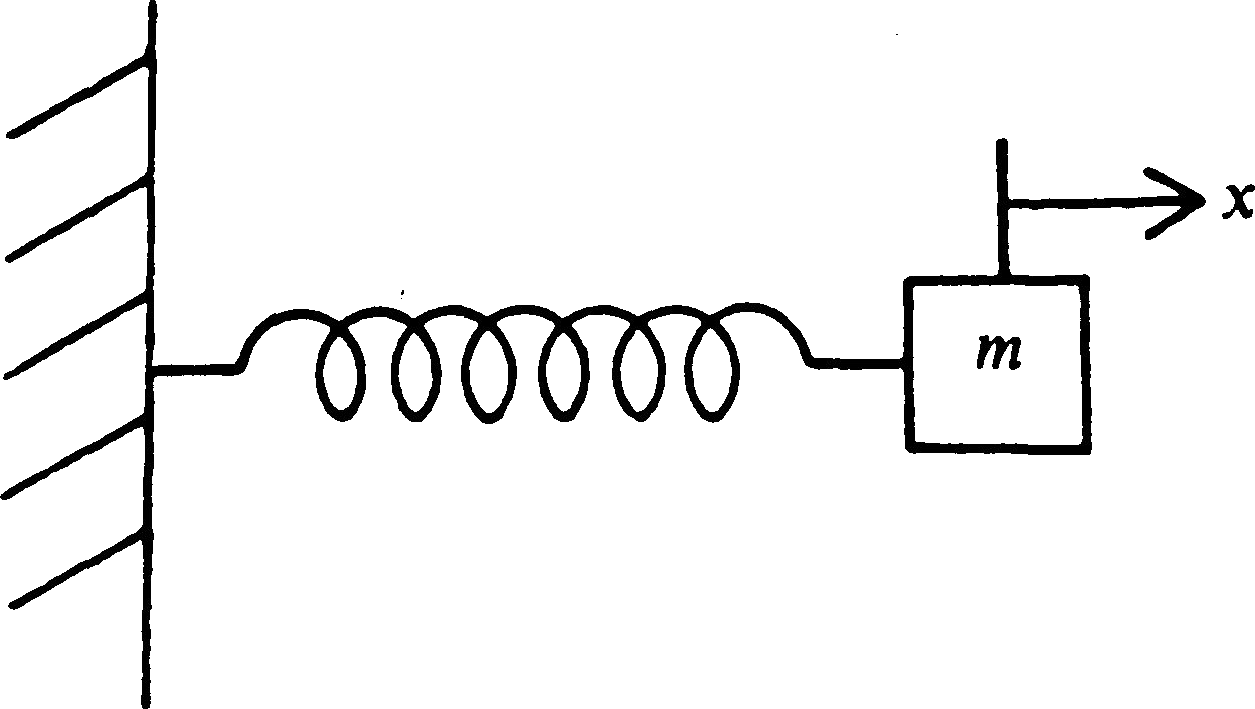
\includegraphics[width=0.5\linewidth]{00_Images/01_chapter/01.png}
    \caption{Simple mass-spring oscillator with mass \( m \), spring stiffness \( K \) and displacement \( x(t) \)}
    \label{fig:simpleosc}
\end{figure}

Consider the prototypical one-dimensional oscillator (as in figure \ref{fig:simpleosc}): a point mass \( m \) attached to a linear spring of stiffness \( K \). Neglecting dissipation, Newton’s second law combined with Hooke’s law yields
\[
m\ddot{x}(t) = - Kx(t)
\quad\Longleftrightarrow\quad
\ddot{x}(t) + \omega_0^2x(t) = 0,
\quad \text{with} \quad
\omega_0 = \sqrt{\frac{K}{m}}
\]
The quantity \( \omega_0 \) is the natural (or eigen) angular frequency of the system and \( f_0 = \omega_0/(2\pi) \) is the corresponding natural frequency. 

\subsection{General Solutions and Initial Conditions}

A complete solution of the homogeneous problem can be written in several equivalent forms, for example
\[
x(t) = A\cos(\omega_0 t + \phi)
\quad\text{or}\quad
x(t) = B\cos(\omega_0 t) + C\sin(\omega_0 t)
\]
where the two independent constants are fixed by the initial state \( (x_0, v_0) = \left(x(0), \dot{x}(0)\right) \). In the cosine-sine form one has \( x_0 = B \) and \( v_0 = \omega_0 C \); in amplitude--phase form,
\[
A = \sqrt{x_0^2 + \left(\frac{v_0}{\omega_0}\right)^2},
\qquad
\phi = \operatorname{atan2}\left( - \frac{v_0}{\omega_0},x_0\right)
\]
For completeness, the kinematic fields follow by differentiation:
\[
v(t) = \dot{x}(t) = - \omega_0 A \sin(\omega_0 t + \phi), 
\qquad
a(t) = \ddot{x}(t) = - \omega_0^2 A \cos(\omega_0 t + \phi) = -\omega_0^2 x(t)
\]
The velocity leads the displacement by \( \pi/2 \) and the acceleration is in antiphase with the displacement, as illustrated in figure \ref{fig:phasekin}. The motion is strictly periodic with period
\[
T = \frac{2\pi}{\omega_0}
\]
so that \( x(t + T) = x(t) \) for all \( t \).

\begin{figure}[!htb]
    \centering
    
\includegraphics[width=0.9\linewidth]{00_Images/01_chapter/02.png}
    \caption{Phase relations between \(x(t)\), \(v(t)\), and \(a(t)\) in harmonic motion}
    \label{fig:phasekin}
\end{figure}

\paragraph{Phase computation:} To determine the initial phase \( \phi \) from the initial state \( (x_0,v_0) \) of the harmonic oscillator \( x(t) = A\cos(\omega_0 t + \phi) \), one needs both \( \cos\phi = x_0/A \) and \( \sin\phi = - v_0/(A\omega_0) \). The ordinary inverse tangent \( \tan^{ - 1}(y/x) \) cannot resolve the correct quadrant of \( \phi \) and fails when \( x = 0 \). The two-argument function \( \operatorname{atan2}(y,x) \) returns the principal argument in \( ( - \pi,\pi] \) using the signs of \( x \) and \( y \), thus removing these ambiguities. Identifying the complex phasor \( \widetilde{A} = A e^{j\phi} = x_0 - j\frac{v_0}{\omega_0} \), one has \( \phi = \arg(\widetilde{A}) = \operatorname{atan2}\left( - \frac{v_0}{\omega_0},x_0\right) \). This is the computational counterpart of the complex-analytic principal argument and provides a numerically robust phase estimate consistent with the geometry of the initial data.

\section{Complex Exponential Representation}

It is often advantageous to represent sinusoidal motion using complex exponentials. Writing
\[
x(t) = A\cos(\omega_0 t + \phi) 
 = \Re\left[A e^{j\phi} e^{j\omega_0 t}\right] 
 = \Re\left[\widetilde{A} e^{j\omega_0 t}\right], 
\quad \text{with} \quad
\widetilde{A} = Ae^{j\phi}
\]
time differentiation becomes algebraic:
\[
v(t) = \left[j\omega_0 \widetilde{A}e^{j\omega_0 t}\right] = j\omega_0 x(t),
\qquad
a(t) = \left[(j\omega_0)^2 \widetilde{A}e^{j\omega_0 t}\right] = - \omega_0^2 x(t)
\]
In this form, differentiation corresponds to multiplication by \( j\omega_0 \), while integration corresponds to multiplication by \( 1/(j\omega_0) \).

\section{Linear Superposition of Harmonic Motions}

Many motions of practical interest are sums of a few simple harmonic oscillations. Because the governing dynamics are linear in the small–amplitude regime, displacements add algebraically and the resulting waveform can often be recast in a compact amplitude–phase form. Two representative cases are especially useful.

\subsection{Components at the Same Frequency}

Consider a family of cosines at the same angular frequency \( \omega_0 \),
\[
x(t) = \sum_{n = 1}^{N} A_n \cos\left(\omega_0 t + \phi_n\right)
\]
Introducing phasors \( \widetilde{A}_n = A_n e^{j\phi_n} \), the sum is a single cosine
\[
x(t) = A\cos\left(\omega_0 t + \phi\right)
\]
with resultant amplitude and phase
\[
A = \sqrt{\left(\sum_n A_n\cos\phi_n\right)^2 + \left(\sum_n A_n\sin\phi_n\right)^2},
\quad
\phi = \operatorname{atan2}\left(\sum_n A_n\sin\phi_n,\ \sum_n A_n\cos\phi_n\right)
\]
This recasting expresses vector addition in the complex plane.

\subsection{Two Components at Nearly Equal Frequencies (Beats)}

Let
\[
x(t) = A_1 \cos\left( \omega_1 t + \phi_1 \right) + A_2 \cos\left( (\omega_1 + \Delta \omega) t + \phi_2 \right),
\qquad 0 < \Delta\omega \ll \omega_1
\]
One may rewrite \( x(t) \) as a slowly modulated cosine at carrier \( \omega_1 \),
\[
x(t) = A(t)\cos\left(\omega_1 t + \phi(t)\right)
\]
where the slowly varying envelope \( A(t) \) and phase \( \phi(t) \) are
\[
A(t) = \sqrt{A_1^{2} + A_2^{2} + 2A_1A_2 \cos\left(\phi_1 - \phi_2 - \Delta \omega t\right)}
\]
\[
\phi(t) = \operatorname{atan2}\left( A_1 \sin \phi_1 + A_2 \sin \left( \phi_2 + \Delta \omega t \right), 
A_1 \cos \phi_1 + A_2 \cos \left( \phi_2 + \Delta \omega t \right) \right)
\]
The instantaneous amplitude varies between \( |A_1 - A_2| \) and \( A_1 + A_2 \) at the beat angular frequency \( \Delta\omega \) (beat frequency \( f_b = \Delta\omega/2\pi \)). In the symmetric special case \( A_1 = A_2 = A \) and \( \phi_1 = \phi_2 = 0 \),
\[
A(t) = A \sqrt{ 2 + 2 \cos( \Delta \omega t)} = 2 A \left| \cos \left( \frac{\Delta \omega}{2} t \right) \right|
\]
so that the envelope periodically collapses to zero and recovers to \( 2A \), producing the familiar beat pattern shown in figure \ref{fig:beats}.

\begin{figure}[!htb]
    \centering
    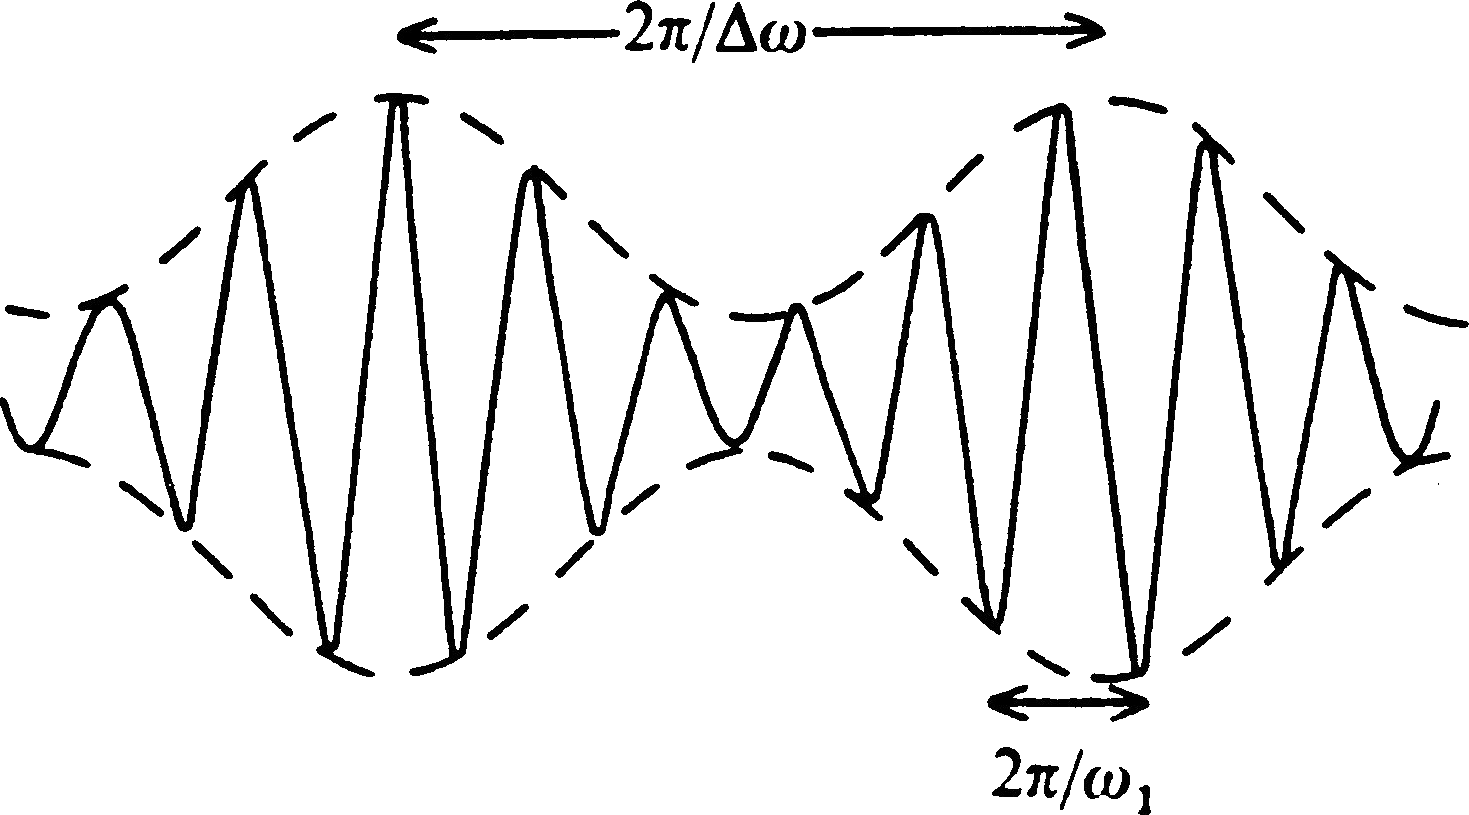
\includegraphics[width=0.5\linewidth]{00_Images/01_chapter/03.png}
    \caption{Beat waveform from the superposition of two nearly equal frequencies}
    \label{fig:beats}
\end{figure}

Importantly, this linear superposition contains only spectral lines at \( \omega_1 \) and \( \omega_1 + \Delta\omega \); it is not amplitude modulation in the nonlinear sense (which would also generate sidebands at \( \omega_1\pm \tfrac{\Delta\omega}{2} \)).

\section{Combinations of Springs and Masses}

When multiple springs act on the same degree of freedom, they may be reduced to an equivalent single spring. The most common layouts are summarized in figure \ref{fig:springcomb}. Two springs in parallel add their stiffnesses,
\[
K_P = K_1 + K_2
\]
whereas two in series combine as
\[
K_S = \frac{K_1K_2}{K_1 + K_2}
\]

\begin{figure}[!htb]
    \centering
    
\includegraphics[width=0.7\linewidth]{00_Images/01_chapter/04.png}
    \caption{Series and parallel combinations of springs and masses}
    \label{fig:springcomb}
\end{figure}

For equal springs \( K_1 = K_2 = K \) one finds \( K_{P} = 2K \) and \( K_{S} = K/2 \). These reductions allow many one-degree-of-freedom mass-spring layouts to be analyzed by substituting an effective stiffness \( K_{\text{eq}} \) and mass \( m_{\text{eq}} \) into
\[
\omega_0 = \sqrt{\frac{K_{\text{eq}}}{m_{\text{eq}}}},\qquad
f_0 = \frac{\omega_0}{2\pi}
\]

\section{Multidimensional Discrete Systems}

Real instruments and engineered structures seldom vibrate as a single lumped mass. A minimal example with more than one coordinate is the coupled two-mass system in figure \ref{fig:2dof}, which already exhibits multiple normal modes and distinct resonance features.

\begin{figure}[!htb]
    \centering
    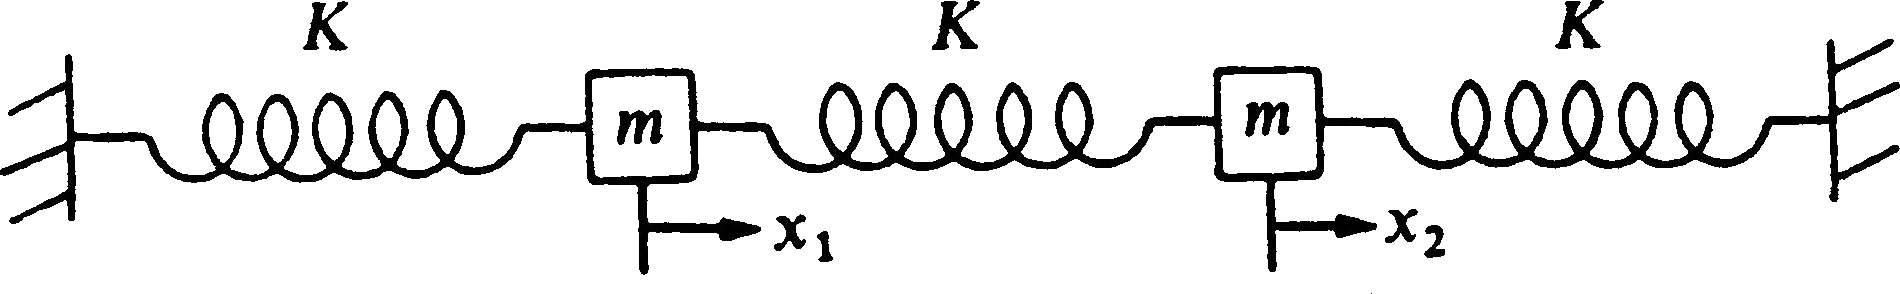
\includegraphics[width=0.5\linewidth]{00_Images/01_chapter/05.png}
    \caption{Two-degree-of-freedom mass-spring system}
    \label{fig:2dof}
\end{figure}

When multiple points can move, the dynamics are captured by the matrix form of Newton’s law for a linear, conservative, discrete system:
\[
\symbf{M} \vv{\ddot{\xi}}(t) + \symbf{K} \vv{\xi}(t) = \symbf{0}
\]
where \( \vv{\xi}(t) \in \mathbb{R}^{N} \) collects the generalized displacements of the \( N \) vibrating coordinates, \( \symbf{M}\in\mathbb{R}^{N\times N} \) is the symmetric mass matrix and \( \symbf{K} \in \mathbb{R}^{N\times N} \) is the symmetric stiffness matrix. Introducing the state vector \( \symbf{w} = [ \vv{\xi}^{T}  \vv{\dot{\xi}}^{T}]^{T} \) and the block matrix
\[
\symbf{\mathcal{M}_K} = 
\begin{bmatrix}
\symbf{0} & \symbf{I} \\
 - \symbf{M}^{ - 1}\symbf{K} & \symbf{0}
\end{bmatrix}
\]
the second-order system is embedded in first-order form \( \dot{\symbf{w}} = \symbf{\mathcal{M}_K} \symbf{w} \).

\subsection{Modal (Eigen) Analysis}

Normal modes arise from the eigenproblem of \( \symbf{\mathcal{M}_K} \). Seeking solutions \( \symbf{w}(t) = \vv{u}e^{\lambda t} \) with \( \symbf{\mathcal{M}_K} \vv{u} = \lambda \vv{u} \) and eliminating velocities yields the generalized eigenvalue problem in configuration space
\[
\symbf{K} \vv{\phi} = - \lambda^{2} \symbf{M} \vv{\phi}
\]
Writing \( \omega^{2} = - \lambda^{2} \ge 0 \), the natural (angular) frequencies \( \omega_n \) are the (real) roots of the characteristic equation
\[
\det \left( - \omega^{2}\symbf{M} + \symbf{K} \right) = 0
\]
with associated nontrivial eigenvectors (mode shapes) \( \vv{\phi}_n \) solving \( \left( - \omega_n^{2} \symbf{M} + \symbf{K} \right) \vv{\phi}_n = \vv{0} \). For conservative systems, the spectrum is finite (size \( N \)) and real. Mode shapes are defined up to a nonzero scalar factor.

\paragraph{Orthogonality and Consequences} Distinct modes \( m\neq n \) satisfy the orthogonality relations
\[
\vv{\phi}_n^{T} \symbf{M} \vv{\phi}_m = 0,
\qquad
\vv{\phi}_n^{T} \symbf{K} \vv{\phi}_m = 0
\]
which express that inertia and stiffness forces associated with one eigenmode do not do work in the motion of another-an energetic decoupling that underpins the mechanical independence of modes. Orthogonality and the resulting diagonalization in modal coordinates, strictly hold for undamped systems; with light proportional damping it remains approximately valid. Any motion can be expanded onto the modal basis, \( \vv{\xi}(t) = \sum_{n = 1}^{N} \vv{\phi}_nq_n(t) \), yielding \( N \) uncoupled scalar oscillators in the modal coordinates \( q_n(t) \).

\section{Damped Oscillations}

Real oscillators exhibit losses due to internal friction, radiation or other dissipation mechanisms. For a single degree of freedom with mass \( m \), viscous damping coefficient \( R \) and stiffness \( K \), the equation of motion reads
\[
m \ddot{x} + R \dot{x} + K x = 0
\quad \Longleftrightarrow \quad
\ddot{x} + 2 \alpha \dot{x} + \omega_0^{2} x = 0
\]
with \( \alpha = R/(2m) \) the (linear) damping rate and \( \omega_0 = \sqrt{K/m} \) the undamped natural angular frequency. Seeking exponential solutions \( x(t) = \widetilde{A} e^{\gamma t} \) gives the characteristic equation \( \gamma^{2} + 2 \alpha \gamma + \omega_0^{2} = 0 \), hence
\[
\gamma = - \alpha \pm j \omega_d,
\qquad
\omega_d = \sqrt{\omega_0^{2} - \alpha^{2}}
\]
For the underdamped case (\( 0 < \alpha < \omega_0 \)), the displacement is a decaying sinusoid,
\[
x(t) = e^{ - \alpha t} \left( A \cos \omega_d t + B \sin \omega_d t \right)
 = A_0 e^{ - \alpha t} \cos \left( \omega_d t + \phi \right)
\]
with constants fixed by the initial state \( (x_0,v_0) \). A convenient form is obtained by setting \( t = 0 \) in \( x \) and \( \dot{x} \):
\[
x(t) = e^{ - \alpha t} \left[ x_0 \cos(\omega_d t) + \frac{v_0 + \alpha x_0}{\omega_d} \sin(\omega_d t) \right]
\]
The motion is not strictly periodic, but the zero-crossing interval (and the interval between successive extrema) remains equal to the damped period \( T_d = 2\pi/\omega_d \). In many mechanical and acoustical systems of interest the damping is light, \( \alpha \ll \omega_0 \), so that \( \omega_d\simeq\omega_0 \). For \( \alpha = \omega_0 \) the system is critically damped and returns to equilibrium without oscillation; for \( \alpha > \omega_0 \) it is overdamped and exhibits a purely exponential relaxation governed by two real rates. The qualitative effect of increasing damping is summarized in figure \ref{fig:dampedcases}.

\begin{figure}[!htb]
    \centering
    
\includegraphics[width=0.9\linewidth]{00_Images/01_chapter/06.png}
    \caption{Free response for increasing damping: underdamped, critical, overdamped}
    \label{fig:dampedcases}
\end{figure}

\subsection{Decay Time and Quality Factor}

The amplitude envelope decays as \( e^{ - \alpha t} \). The decay time (or relaxation time) \( \tau \) is the time for the amplitude to drop by a factor \( e \), namely
\[
\tau = \frac{1}{\alpha} = \frac{2m}{R}
\]
An equivalent and widely used metric is the (dimensionless) quality factor \( Q \), which compares reactive to resistive effects and, for a lightly damped second-order resonator, is
\[
Q = \frac{\omega_0}{2\alpha} = \frac{K}{R\omega_0}
\]
Via \( \alpha = \omega_0/(2Q) \), the envelope over one (damped) period \( T_d \) decreases by the factor \( e^{ - \alpha T_d} \approx e^{ - \pi/Q} \) when \( \alpha \ll \omega_0 \). Typical values in musical acoustics span orders of magnitude: woodwind bores and wooden soundboards often exhibit \( Q \) between a few tens and a few hundreds, whereas plucked and struck strings can reach \( Q\sim10^{2} - 10^{4} \), depending on frequency range and construction. These figures reflect that each resonance behaves approximately as a single resonator with its own \( Q \).

\section{Air Resonators and Helmholtz Resonance}

Confined air can behave as an elastic element, storing and releasing potential energy through reversible compression. Simple archetypes, an air-filled cylinder closed by a moving piston and the Helmholtz resonator, admit compact lumped models that map pressure–volume dynamics onto the mass–spring oscillator. These models provide closed-form expressions for resonance frequencies in terms of geometry and thermophysical constants. Figure \ref{fig:helmholtzschemes} summarizes the key geometries and their mechanical analogies: a piston-cylinder resonator, the classical Helmholtz resonator with a neck, and a neckless cavity resonance.

\begin{figure}[!htb]
    \centering
    
\includegraphics[width=0.9\linewidth]{00_Images/01_chapter/07.png}
    \caption{Lumped-element analogies for air resonators: piston, Helmholtz, and neckless cavity}
    \label{fig:helmholtzschemes}
\end{figure}

\subsection{Piston in a Rigid Cylinder}

Consider a frictionless piston of mass \( m \) and area \( S \) sliding in a rigid, airtight cylinder of length \( L \). A small axial displacement changes the enclosed volume by \( \Delta V = Sx \) and produces a restoring pressure proportional to the fractional volume change. Under adiabatic conditions the effective (air) spring constant is
\[
K = \gamma p_a\frac{S}{L}
\]
where \( p_a \) is the ambient pressure and \( \gamma\simeq 1.4 \) is the ratio of specific heats for air. The piston–air system is thus a single-degree-of-freedom oscillator with natural frequency
\[
f_0 = \frac{1}{2\pi}\sqrt{\frac{K}{m}}
 = \frac{1}{2\pi}\sqrt{\frac{\gamma p_aS}{mL}}
\]
The dependence \( f_0\propto \sqrt{S/L} \) highlights that enlarging the cylinder (larger \( L \)) softens the effective spring, while increasing the piston area (larger \( S \)) stiffens it.

\subsection{Helmholtz Resonator with a Neck}

A Helmholtz resonator comprises a cavity of volume \( V \) vented by a short neck of length \( L \) and cross-section \( S \). The air slug in the neck behaves as the inertial mass
\[
m = \rho SL
\]
with \( \rho \) the air density, while the cavity acts as an acoustic spring with stiffness
\[
K = \rho\frac{S^{2}c^{2}}{V}
\]
where \( c \) is the speed of sound. The resonance frequency follows directly:
\[
f_0 = \frac{1}{2\pi}\sqrt{\frac{K}{m}}
 = \frac{c}{2\pi}\sqrt{\frac{S}{VL}}
\]
In this model, making the neck narrower (smaller \( S \)) lowers the resonance because the spring constant scales with \( S^2 \) while the inertial mass scales with \( S \), so the ratio \( K/m\propto S \) decreases.

\subsection{Neckless (Aperture) Resonator and End Correction}

When the cavity opens directly to the exterior without a physical neck, a virtual neck arises because a finite plug of exterior air moves in concert with the flow at the aperture. For a flanged circular opening of radius \( a \), the effective neck length is well approximated by twice the end correction \( \ell_e = \tfrac{8}{3\pi}a\approx 0.85a \), giving \( L_{\mathrm{eff}}\approx 2\ell_e\approx 1.7a \) for a large surrounding face. The corresponding neck mass and resonance frequency are then
\[
m = \rho SL_{\mathrm{eff}}
 = \rho(\pi a^{2})\left(\frac{16}{3\pi}a\right)
 = 5.33\rho a^{3},
\qquad
f_0 = \frac{c}{2\pi}\sqrt{\frac{1.85a}{V}}
\]
where the numerical factors reflect the end-correction geometry. If the baffle (face) around the hole is not large, the effective length is smaller and the actual frequency is slightly higher than this large-baffle estimate. 

\paragraph{Geometry note} The end correction depends on whether the opening is flanged or unflanged. Typical low-frequency values are \( \Delta L \approx 0.82a \) (flanged) and \( \Delta L \approx 0.61a \) (unflanged), so mixed conditions lead to intermediate \( L_{\mathrm{eff}} \).

\section{Forced Oscillations and Frequency Response Functions}

Free vibrations describe how a system evolves from an initial state. In musical acoustics, however, the most relevant situation is often the opposite: the resonator is driven by an external excitation (a bow force, an impact, an airflow perturbation) and we are interested in its steady-state response as a function of frequency. 

\subsection{Steady-State Harmonic Response}

\begin{figure}[!htb]
    \centering
    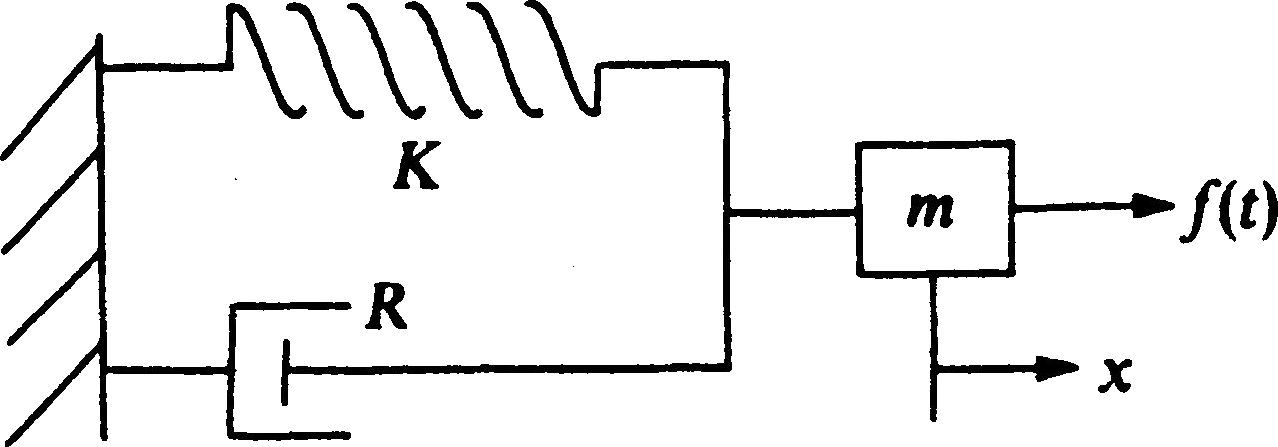
\includegraphics[width=0.5\linewidth]{00_Images/01_chapter/08.png}
    \caption{Damped oscillator driven by an external force \(F(t)\)}
    \label{fig:forcedosc}
\end{figure}

Let us consider the damped oscillator (figure \ref{fig:forcedosc}) driven by a sinusoidal force,
\[
m\ddot{x}(t) + R\dot{x}(t) + Kx(t) = F e^{j\omega t}
\]
Since the dynamics are linear, the steady-state response is harmonic at the same angular frequency \( \omega \). Introducing the complex ansatz
\[
x(t) = X(\omega)e^{j\omega t}
\]
substitution yields
\[
\left(K - \omega^{2}m + j\omega R\right)X(\omega) = F
\qquad\Rightarrow\qquad
X(\omega) = \frac{F}{K - \omega^{2}m + j\omega R}
\]
It is convenient to normalize by the mass and define
\[
\omega_0^2 = \frac{K}{m},\qquad \alpha = \frac{R}{2m}
\]
so that the displacement phasor becomes
\[
X(\omega) = \frac{F/m}{\omega_0^{2} - \omega^{2} + j2\alpha\omega}
\]
This is the frequency-domain description of the forced damped oscillator and it makes phase and amplitude immediately accessible.

\subsection{Mechanical Impedance and Mobility}

A particularly meaningful response quantity is the mechanical impedance, defined as the ratio between applied force and resulting velocity. Since
\[
V(\omega) = \dot{x}(t)e^{ - j\omega t} = j\omega \widetilde{X}(\omega)
\]
the impedance is
\[
Z(\omega) = \frac{F}{V(\omega)}
 = \frac{F}{j\omega X(\omega)}
 = R + j\left(\omega m - \frac{K}{\omega}\right)
 = R + jX(\omega)
\]
The real part \( R \) is the mechanical resistance, while the imaginary part is the mechanical reactance. The reactance crosses zero at resonance, since
\[
X(\omega_0) = \omega_0 m - \frac{K}{\omega_0} = 0
\]
and consequently, the impedance magnitude has a minimum around \( \omega = \omega_0 \). The inverse quantity
\[
Y(\omega) = \frac{1}{Z(\omega)} = \frac{V(\omega)}{F}
\]
is the mobility (or admittance). Writing \( Y = G + jB \), \( G \) is the conductance and \( B \) is the susceptance. Mobility is widely used in musical acoustics because radiated sound pressure is closely related to the vibrational velocity of the radiating surfaces. Typical trends of these quantities across resonance, together with the Nyquist representation, are illustrated in figure \ref{fig:impedance_mobility}.

\begin{figure}[!htb]
    \centering
    
\includegraphics[width=0.7\linewidth]{00_Images/01_chapter/09.png}
    \caption{Impedance and mobility of a damped oscillator in the frequency domain}
    \label{fig:impedance_mobility}
\end{figure}

\subsection{A Family of Vibrational FRFs}

Impedance and mobility are two members of a broader family of vibrational frequency response functions (FRFs), obtained by taking different output variables over the same input force:

\begin{align*}
&\Theta(\omega) = \frac{X(\omega)}{F(\omega)} \quad &\text{(receptance)}, 
\qquad
&\Sigma(\omega) = \frac{F(\omega)}{X(\omega)} \quad &\text{(dynamic stiffness)}
\\
&Y(\omega) = \frac{\dot{X}(\omega)}{F(\omega)} \quad &\text{(mobility)}, 
\qquad
&Z(\omega) = \frac{F(\omega)}{\dot{X}(\omega)} \quad &\text{(impedance)}
\\
&I(\omega) = \frac{\ddot{X}(\omega)}{F(\omega)} \quad &\text{(inertance)}, 
\qquad
&M(\omega) = \frac{F(\omega)}{\ddot{X}(\omega)} \quad &\text{(apparent mass)}
\end{align*}

In what follows, impedance and mobility will be emphasized, as they provide a direct link to velocity-driven sound radiation mechanisms. 

\subsection{Static Displacement, Resonance Gain and Asymptotic Behavior}

If the system is subject to a constant force \( F \), the static displacement is
\[
x_s = \frac{F}{K}
\]
At resonance (\( \omega = \omega_0 \)), it can be shown that the oscillation amplitude scales as
\[
|x(\omega_0)| = Qx_s
\]
so that the quality factor \( Q \) acts as an amplification factor of the static displacement. The reactance term in the impedance,
\[
X(\omega) = \omega m - \frac{K}{\omega}
\]
It also provides a useful physical interpretation. For \( \omega > \omega_0 \) the reactance is positive and dominated by \( \omega m \); hence, the system behaves mass-like. For \( \omega < \omega_0 \) the reactance is negative and dominated by \( - K/\omega \); hence, the system behaves spring-like. This is a general feature of second-order resonators: above resonance, they act as masses; below resonance, as springs.

\subsection{Receptance Bandwidth and the Q Factor}

The receptance of the damped oscillator has the characteristic form
\[
\Theta(\omega) = \frac{X(\omega)}{F(\omega)}
\propto
\frac{1}{\omega^{2} - 2j\alpha\omega - \omega_0^{2}}
\]
whose magnitude reaches a maximum near the damped resonance \( \omega = \omega_d \). Moreover, the magnitude drops by \SI{3}{\decibel} at
\[
\omega = \omega_d \pm \alpha
\]
so that the quantity \( 2 \alpha \) has the meaning of the (angular) bandwidth of the response:
\[
\Delta\omega \simeq 2\alpha
\]
Therefore, the quality factor
\[
Q = \frac{\omega_0}{2\alpha}
\]
can be interpreted as the ratio between the central frequency and the bandwidth (high \( Q \): sharp resonance; low \( Q \): broad resonance).

\subsection{Transient Response to a Suddenly Applied Harmonic Force}

The frequency response functions introduced above describe the steady-state motion under a harmonic excitation. In practice, however, the forcing is often applied at a finite time (e.g., an actuator is switched on at \( t = 0 \)), so the response generally contains a transient component in addition to the steady-state solution. Consider the damped oscillator driven by a sinusoidal force applied suddenly at rest,
\[
m\ddot{x}(t) + R\dot{x}(t) + Kx(t) = F\cos(\omega t) u(t)
\]
where \( u(t) \) is the Heaviside step. By linearity, the displacement can be written as the sum
\[
x(t) = x_{\mathrm{tr}}(t) + x_{\mathrm{ss}}(t)
\]
where \( x_{\mathrm{tr}} \) solves the homogeneous equation (free decay) and \( x_{\mathrm{ss}} \) is a particular (steady-state) solution at the driving frequency. For the underdamped case, the transient has the standard decaying oscillatory form
\[
x_{\mathrm{tr}}(t) = A e^{ - \alpha t} \cos\left(\omega_d t + \phi\right),
\qquad
\omega_d = \sqrt{\omega_0^2 - \alpha^2},
\qquad
\alpha = \frac{R}{2m}
\]
and, for light damping, \( \omega_d \simeq \omega_0 \). The steady-state motion is harmonic at the forcing frequency and may be written in amplitude-phase form as
\[
x_{\mathrm{ss}}(t) = X(\omega)\sin\left(\omega t + \varphi\right),
\qquad
X(\omega) = \frac{F}{\omega|Z(\omega)|}
\]
where \( Z(\omega) = R + j \left(\omega m - \frac{K}{\omega}\right) \) is the mechanical impedance. Therefore, the overall response can be expressed compactly as
\[
x(t) = A e^{ - \alpha t} \cos(\omega_d t + \phi) + \frac{F}{\omega|Z(\omega)|} \sin(\omega t + \varphi)
\]
Representative time histories for different values of \(\omega/\omega_0\) are shown in figure \ref{fig:sudden_sine}.

\begin{figure}[!htb]
    \centering
    
\includegraphics[width=0.7\linewidth]{00_Images/01_chapter/10.png}
    \caption{Response to a sinusoid applied suddenly at \( t = 0 \) for different \( \omega/\omega_0 \)}
    \label{fig:sudden_sine}
\end{figure}

\paragraph{Beatings and build-up} During the transient, the displacement exhibits components at the natural frequency (approximately \( f_0 \)) and at the driving frequency \( f = \omega/2\pi \). If \( f \) is close enough to \( f_0 \), the superposition of these two oscillatory components produces beatings in the observed waveform. As damping increases, the natural-frequency component decays faster and beatings disappear more quickly. In the special case \( \omega = \omega_0 \), the response builds up to the steady-state solution without beats: regardless of the initial transient details, the motion eventually settles into the forced oscillation at frequency \( \omega \).

\section{Forced Multidimensional Discrete Systems}

When a multidimensional discrete system is excited by a distribution of external forces, its motion is governed by the forced matrix equation
\[
\symbf{M}\vv{\ddot{\xi}}(t) + \symbf{K}\vv{\xi}(t) = \vv{f}(t)
\]
Spectral theory ensures that the eigenmodes of the associated conservative system form a complete basis for the space spanned by \( \vv{\xi} \). As a consequence, any response admits a unique expansion onto the modal basis,
\[
\vv{\xi}(t) = \sum_{n = 1}^{N}\vv{\phi}_n q_n(t)
\]
where \( q_n(t) \) are the generalized displacements, also referred to as modal participation factors. 

\subsection{Undamped Case: Modal Forces and Resonant FRFs}

Substituting the modal expansion into the forced equation of motion and taking the inner product with an eigenvector \( \vv{\phi}_m \) orthogonality eliminates cross-terms and yields one scalar oscillator per mode:
\[
\langle \vv{\phi}_n,\symbf{M}\vv{\phi}_n\rangle \ddot{q}_n(t)
 + \langle \vv{\phi}_n,\symbf{K}\vv{\phi}_n\rangle q_n(t)
 = \langle \vv{\phi}_n,\vv{f}(t)\rangle
\]
It is natural to introduce the modal quantities
\[
m_n = \langle \vv{\phi}_n,\symbf{M}\vv{\phi}_n\rangle,
\qquad
\kappa_n = \langle \vv{\phi}_n,\symbf{K}\vv{\phi}_n\rangle,
\qquad
f_n(t) = \langle \vv{\phi}_n,\vv{f}(t)\rangle
\]
so that, using \( \kappa_n = m_n\omega_n^2 \), each modal coordinate satisfies
\[
\ddot{q}_n(t) + \omega_n^2 q_n(t) = \frac{f_n(t)}{m_n}
\]
The scalar forcing term \( f_n \) is the projection of the force distribution onto mode \( n \): if \( f_n(t) = 0 \), then mode \( n \) cannot be excited by that forcing. Physically, this occurs, for instance, when a string drives a soundboard at a point coinciding with a nodal line of a given soundboard mode. In the frequency domain, for a harmonic forcing at angular frequency \( \omega \), the modal receptance reads
\[
Q_n(\omega) = \frac{f_n(\omega)}{m_n} \frac{1}{\omega_n^2 - \omega^2}
\]
and the configuration-space response becomes a sum of resonant terms,
\[
\vv{\Xi}(\omega) = \sum_{n = 1}^{N} \vv{\phi}_n\frac{f_n(\omega)}{m_n} \frac{1}{\omega_n^2 - \omega^2}
\]
Consequently, if the system is forced at a frequency \( \omega \) close to a given eigenfrequency \( \omega_n \), that modal contribution dominates and (in the ideal undamped limit) its amplitude tends to infinity.

\paragraph{Normalization invariance} Because each eigenvector is defined up to a multiplicative constant \( C \), one has \( m_n \propto C^2 \) while \( f_n \propto C \), hence \( q_n \propto C^{ - 1} \). The physical displacement \( \vv{\xi} = \sum_n \vv{\phi}_n q_n \) is therefore independent of the chosen normalization of the mode shapes. 

\subsection{Damped Case: Modal Coupling and Weak-Damping Correction}

In a linear system with a finite number of degrees of freedom, viscous dissipation can be modeled as a non-negative quadratic form of the velocity,
\[
\mathcal{D}(\vv{\dot{\xi}}) = \frac{1}{2}\vv{\dot{\xi}}^{T}\symbf{C}\vv{\dot{\xi}}
\]
where \( \symbf{C} \) is a symmetric damping matrix. The forced equations of motion then become
\[
\symbf{M}\vv{\ddot{\xi}}(t) + \symbf{C}\vv{\dot{\xi}}(t) + \symbf{K}\vv{\xi}(t) = \vv{F}(t)
\]
Expanding \( \vv{\xi}(t) = \sum_m \vv{\phi}_m q_m(t) \) onto the conservative eigenmodes and projecting onto \( \vv{\phi}_n \) yields
\[
\langle \vv{\phi}_n,\symbf{M}\vv{\phi}_n\rangle \ddot{q}_n
 + \sum_{m}\langle \vv{\phi}_n,\symbf{C}\vv{\phi}_m\rangle \dot{q}_m
 + \langle \vv{\phi}_n,\symbf{K}\vv{\phi}_n\rangle q_n
 = \langle \vv{\phi}_n,\vv{F}\rangle
\]
Defining the inter-modal damping coefficients through
\[
\langle \vv{\phi}_n,\symbf{C}\vv{\phi}_m\rangle = 2\zeta_{mn}m_n\omega_n
\]
one obtains the coupled system for the generalized coordinates.
\[
\ddot{q}_n + 2\omega_n\sum_{m}\zeta_{mn}\dot{q}_m + \omega_n^2 q_n
 = \frac{f_n}{m_n}
\]
In general, \( \symbf{C} \) cannot be diagonalized in the same basis as \( \symbf{M} \) and \( \symbf{K} \), so \( \zeta_{mn} \) with \( m \neq n \) are not zero and the modes are coupled through velocity terms. It is common to separate the diagonal (modal) damping coefficient \( \zeta_n \) from the off-diagonal coupling terms, rewriting
\[
\ddot{q}_n + 2\omega_n\zeta_n\dot{q}_n + \omega_n^2 q_n
 = \frac{f_n}{m_n} - 2\omega_n\sum_{m\neq n}\zeta_{mn}\dot{q}_m
\]
Under the assumption of weak damping, one may seek first-order corrections of the conservative eigenpairs,
\[
\omega_n' = \omega_n + \Delta\omega_n,
\qquad
\vv{\phi}_n' = \vv{\phi}_n + \Delta\vv{\phi}_n
\]
leading to the approximation
\[
\Delta\omega_n \simeq j\zeta_n\omega_n
\]
Hence, the correction to the eigenfrequency is purely imaginary: the corresponding eigensolution becomes a damped sinusoid, slowly decaying when damping is weak. Moreover, at first order, the inter-modal damping terms do not affect \( \Delta\omega_n \), which is equivalent to approximating \( \symbf{C} \) as diagonal in the modal basis. Finally, the weak-damping correction to the eigenshapes can be expressed as
\[
\vv{\phi}_n'
 = 
\vv{\phi}_n
 + 
2jm_n\omega_n^2
\sum_{m\neq n}
\vv{\phi}_m
\frac{\zeta_{mn}}{m_m(\omega_n^2 - \omega_m^2)}
\]
If neighboring eigenfrequencies are well separated, the correction remains small (of the order of \( \zeta_{mn} \)); conversely, for closely spaced modes, the denominator \( \omega_n^2 - \omega_m^2 \) can magnify the perturbation and significantly alter the shapes. Since the correction is purely imaginary, the damped mode shapes are no longer everywhere in phase (or in anti-phase) as in the conservative limit. 

\section{Forced Vibration of a Two-Mass System}

A simple yet widely applicable coupled resonator is the two-mass system in which a sinusoidal driving force acts on one mass only. This layout is a prototype for a bass-reflex loudspeaker, a guitar with fixed ribs and the dynamic absorber used to suppress machine vibrations. A particularly important case is the driven two-mass system in figure \ref{fig:twomass_forced}, together with its equivalent electrical circuit representation, which makes clear the close analogy between mechanical and electrical networks.

\begin{figure}[!htb]
    \centering
    
\includegraphics[width=0.7\linewidth]{00_Images/01_chapter/11.png}
    \caption{Driven two-mass system and its electrical analogue}
    \label{fig:twomass_forced}
\end{figure}

\subsection{Equations of Motion}

Let \( x_1(t) \) and \( x_2(t) \) denote the displacements of \( m_1 \) and \( m_2 \). With spring constants \( K_1 \) (to ground) and \( K_2 \) (coupling spring) and a harmonic force \( F_0\sin(\omega t) \) applied to \( m_1 \), the equations of motion are
\[
m_1\ddot{x}_1 + K_1 x_1 + K_2(x_1 - x_2) = F_0 \sin(\omega t),
\qquad
m_2\ddot{x}_2 + K_2(x_2 - x_1) = 0
\]
This is the minimal discrete model in which coupling generates two resonance frequencies, in contrast to the single peak of a one-degree-of-freedom oscillator.

\subsection{Harmonic Solution, Resonances and Antiresonance}

Seeking steady-state solutions at the driving frequency,
\[
x_1(t) = \Re\left\{X_1(\omega)e^{j\omega t}\right\},
\qquad
x_2(t) = \Re\left\{X_2(\omega)e^{j\omega t}\right\}
\]
one obtains the algebraic system
\[
\begin{bmatrix}
K_1 + K_2 - \omega^2 m_1 & - K_2\\
 - K_2 & K_2 - \omega^2 m_2
\end{bmatrix}
\begin{bmatrix}
X_1 \\ X_2
\end{bmatrix}
 = 
\begin{bmatrix}
F_0 \\ 0
\end{bmatrix}
\]
Solving by elimination yields the response amplitudes
\[
X_1(\omega) = 
\frac{(K_2 - \omega^2 m_2)F_0}
{(K_1 + K_2 - \omega^2 m_1)(K_2 - \omega^2 m_2) - K_2^2},
\]
\[
X_2(\omega) = 
\frac{K_2 F_0}
{(K_1 + K_2 - \omega^2 m_1)(K_2 - \omega^2 m_2) - K_2^2}
\]
The common denominator
\[
D(\omega) = (K_1 + K_2 - \omega^2 m_1)(K_2 - \omega^2 m_2) - K_2^2
\]
vanishes at two angular frequencies, producing two resonances (two poles of the FRF), corresponding to the normal modes of the coupled conservative system. In addition, \( X_1 \) has a zero (a notch) when its numerator vanishes:
\[
K_2 - \omega^2 m_2 = 0
\quad\Longrightarrow\quad
\omega = \omega_2 = \sqrt{\frac{K_2}{m_2}}
\]
Thus, the driven mass exhibits an antiresonance at \( \omega = \omega_2 \): despite a nonzero applied force, the steady-state displacement \( X_1 \) cancels by destructive interference through the coupling path.

\paragraph{Dynamic absorber and bass reflex interpretation} In a dynamic absorber, \( m_2 \) and \( K_2 \) are chosen so that \( \omega_2 \approx \omega_1 \) (i.e., the absorber is tuned near the primary resonance). Then the response of the main mass \( m_1 \) is strongly reduced and in the tuned idealized limit the displacement of \( m_1 \) goes to zero at the targeted frequency. The same mechanism underlies the bass-reflex loudspeaker: the enclosure/port resonance restrains the cone motion from diverging by introducing a notch-like cancellation in the cone response. 

\paragraph{Application to plucked-string instruments} A guitar or violin body may be interpreted, at lowest order, as a coupled two-resonator system: the top plate contributes an effective \( (m_1,K_1) \), while the oscillating air plug at the sound hole (together with the cavity compliance) contributes \( (m_2,K_2) \). In that case, \( \omega_2 \) need not coincide with \( \omega_1 \) and the measured mobility typically shows two peaks (the coupled resonances) separated by a dip (the antiresonance). 
